%%%%%%%%%%%%%%%%%%%%%%%%%%%%%%%%%%%%%%%%%%%%%%%%%%%%%%%%%%%%%%%%%%%%%%%%%%%%%%%%
% CVMR Poster Template based on:
% Dreuw & Deselaer's Poster Version 1.0 (11/04/13)
% http://www-i6.informatik.rwth-aachen.de/~dreuw/latexbeamerposter.php
%%%%%%%%%%%%%%%%%%%%%%%%%%%%%%%%%%%%%%%%%%%%%%%%%%%%%%%%%%%%%%%%%%%%%%%%%%%%%%%%

\documentclass[final,hyperref={pdfpagelabels=false}]{beamer}
\usepackage[orientation=portrait,size=a0,scale=1.4]{beamerposter} % Use the beamerposter package for laying out the poster with a portrait orientation and an a0 paper size

\usetheme{cvmr}

\usepackage[english]{babel} % English language/hyphenation
\usepackage{amsmath,amsthm,amssymb,latexsym} % For including math equations, theorems, symbols, etc
\usepackage{enumitem,xcolor}
\usepackage[scaled]{helvet}
\usepackage[percent]{overpic}
\usepackage{microtype}
\setlength{\emergencystretch}{1em}
\usepackage{booktabs} % Top and bottom rules for tables
\usepackage{subfig}
\usepackage[justification=justified]{caption}
\usepackage{adjustbox}
\usepackage[binary-units=true]{siunitx}
\usepackage{tikz}
\usetikzlibrary{shapes,arrows,calc,backgrounds,positioning,fit}
\usepackage[acronym,xindy]{glossaries}
\newacronym{cvmr}{CVMR}{Computer Vision and Mixed Reality}
\newacronym{hsrm}{HSRM}{High-Speed and Robust Monocular}

\newacronym{icarus}{Icarus}{Infrastructure for Compact Aerial Robots Under Supervision}

\newacronym{mav}{MAV}{Micro Aerial Vehicle}
\newacronym{rmse}{RMSE}{Root-Mean-Square Error}
\newacronym{ros}{ROS}{Robot Operating System}
\newacronym{sar}{SAR}{Search and Rescue}
\newacronym{slam}{SLAM}{Simultaneous Localization and Mapping}
\newacronym{ugv}{UGV}{Unmanned Ground Vehicle}


\newcommand{\blocktextwidth}{0.93\textwidth}

% graphics path
\graphicspath{{./figures/}}

% input path
\makeatletter
\providecommand*{\input@path}{}
\edef\input@path{{./figures/}\input@path}% prepend
\makeatother


%---TITLE-----------------------------------------------------------------------

\title{
Comparing raw audio generation algorithms on the task of music generation
} % Poster title

\author{%
Fabian Stahl
} % Author(s)

\institute{%
Computer Vision \& Mixed Reality Group, Hochschule RheinMain University of Applied Sciences, Wiesbaden
} % Institution(s)

%---FOOTER----------------------------------------------------------------------

\newcommand{\leftfoot}{}%http://cvmr.mi.hs-rm.de/icarus} % Left footer text
\newcommand{\rightfoot}{fabian.stahl@student.hs-rm.de} % Right footer text

%-------------------------------------------------------------------------------

\begin{document}

\begin{frame}[t] % The whole poster is enclosed in one beamer frame

\begin{columns}[t] % The whole poster consists of three major columns, each of which can be subdivided further with another \begin{columns} block - the [t] argument aligns each column's content to the top

%%%%%%%%%%%%%%%%%%%%%%%%%%%%%%%%%%%%%%%%%%%%%%%%%%%%%%%%%%%%%%%%%%%%%%%%%%%%%%%%
%        LEFT  COLUMN        %%%%%%%%%%%%%%%%%%%%%%%%%%%%%%%%%%%%%%%%%%%%%%%%%%%
%%%%%%%%%%%%%%%%%%%%%%%%%%%%%%%%%%%%%%%%%%%%%%%%%%%%%%%%%%%%%%%%%%%%%%%%%%%%%%%%

\begin{column}{.31\textwidth} % The first column

%-------------------------------------------------------------------------------

{
\setbeamercolor{block title}{fg=myfg,bg=white} % Change the block title color
\setbeamercolor{block body}{fg=myfg,bg=white} % Change the block title color

%---INTRODUCTION----------------------------------------------------------------

\vspace{0.9em}

\begin{block}{Introduction}
\begin{minipage}[]{\blocktextwidth}

% Motivation
Music can be found in almost every movie, video game or public location.
Its targeted use can change people's mood, encourage buying decisions or add context to accompanying content.
However, composing, recording and mixing music is a creative process, that takes a lot of time and skill to master.
This poses the question, if pleasing music can be generated autonomously.

Deep neural networks have been known to solve a wide range problems.
During this semester's project I will compare different network architectures to generate sample based music, show how they can be trained and rate results.
Some of the most promising candidates can be found in~\cite{deepsound}.

\end{minipage}
\end{block}
}

\vspace{1.655em}

%---Related Work------------------------------------------------------------------
            
\begin{block}{Related Work}
\begin{minipage}[]{\blocktextwidth}
The field of audio generation offers a lot of different research fields.
For example, it was found, that deep neural networks perform excellent in the text-to-speech (TTS) domain~\cite{van2016wavenet, arik2017deep, chung2015recurrent, kalchbrenner2018efficient}.
However, when it comes to music synthesis, these architectures seem to lack the ability to capture long term time structures which results, if not in noise, in rapidly changing motives.

Most approaches to generate music use MIDI data, a binary format specifying musical notes~\cite{yang2017midinet, mogren2016c, tikhonov2017music, hennig2017classifying}.
This symbolic representation makes the format very slim, however the musical interpretation (the raw audio sent to the sound port) is up to an external MIDI synthesizer.

Only few sample based approaches to generate music are known, that generate pleasing results.
The most promising candidates are presented in the following.

%Since most approaches have heavy downsides, there are no clear superior network architectures for this kind of data.
%For example, an already compressed 3 minute mp3 Song is about 3MB.
%Data of this size cannot be fed into most network architectures due to resource limitations.
\end{minipage}
\end{block}

%---CNN----------------------------------------------------------------------------

\begin{block}{CNN-based Approach}
\begin{minipage}[]{\blocktextwidth}
Convolutional Neural Networks (CNNs) are very popular in the field of computer vision because they take into account the spatial structure of input data.
But they are rather uncommon when it comes to sequential data.

However, in 2016 a Microsoft research team presented State-of-the-Art TTS results using a fully convolutional neural network, called \textbf{WaveNet}~\cite{van2016wavenet}.
Dilated convolutions were used to increase the field of perception (see Figure below).
Experiments also included piano music synthesis.
Unfortunately choosing the right hyperparameters for training is quite difficult, generation is slow and training takes several days on a cluster of GPUs.
\begin{figure}[ht]
    \label{fig:wavenet}
    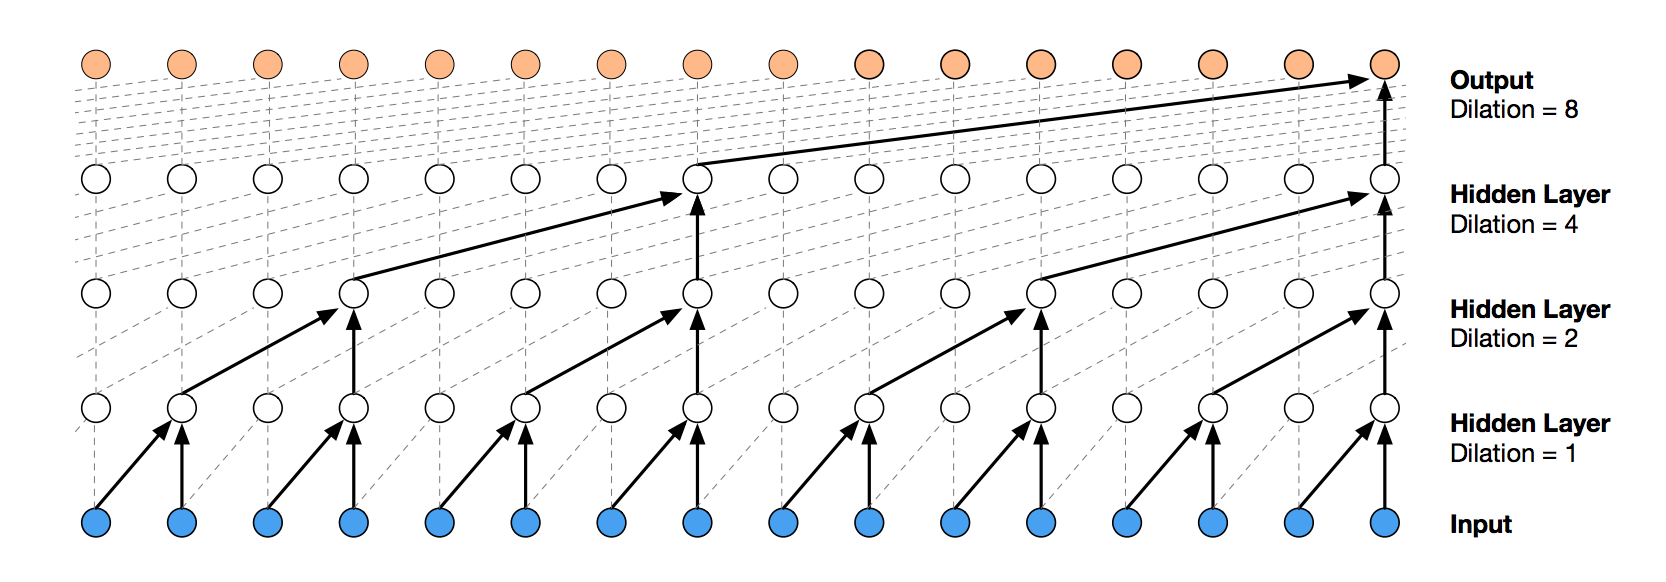
\includegraphics[width=\textwidth]{wavenet-trans.png}
    \caption*{simplified WaveNet architecture}
\end{figure}

%\cite{donahue2018adversarial}
\end{minipage}
\end{block}

%-------------------------------------------------------------------------------

\end{column} % End of the first column

%%%%%%%%%%%%%%%%%%%%%%%%%%%%%%%%%%%%%%%%%%%%%%%%%%%%%%%%%%%%%%%%%%%%%%%%%%%%%%%%
%%%%%%%%%%%%%%%%%%%%%%%%%%%           SPANNED MIDDLE AND RIGHT COLUM           %
%%%%%%%%%%%%%%%%%%%%%%%%%%%%%%%%%%%%%%%%%%%%%%%%%%%%%%%%%%%%%%%%%%%%%%%%%%%%%%%%


\begin{column}{0.6375\textwidth} % The second column

\begin{figure}[ht]
    \label{fig:robot}
    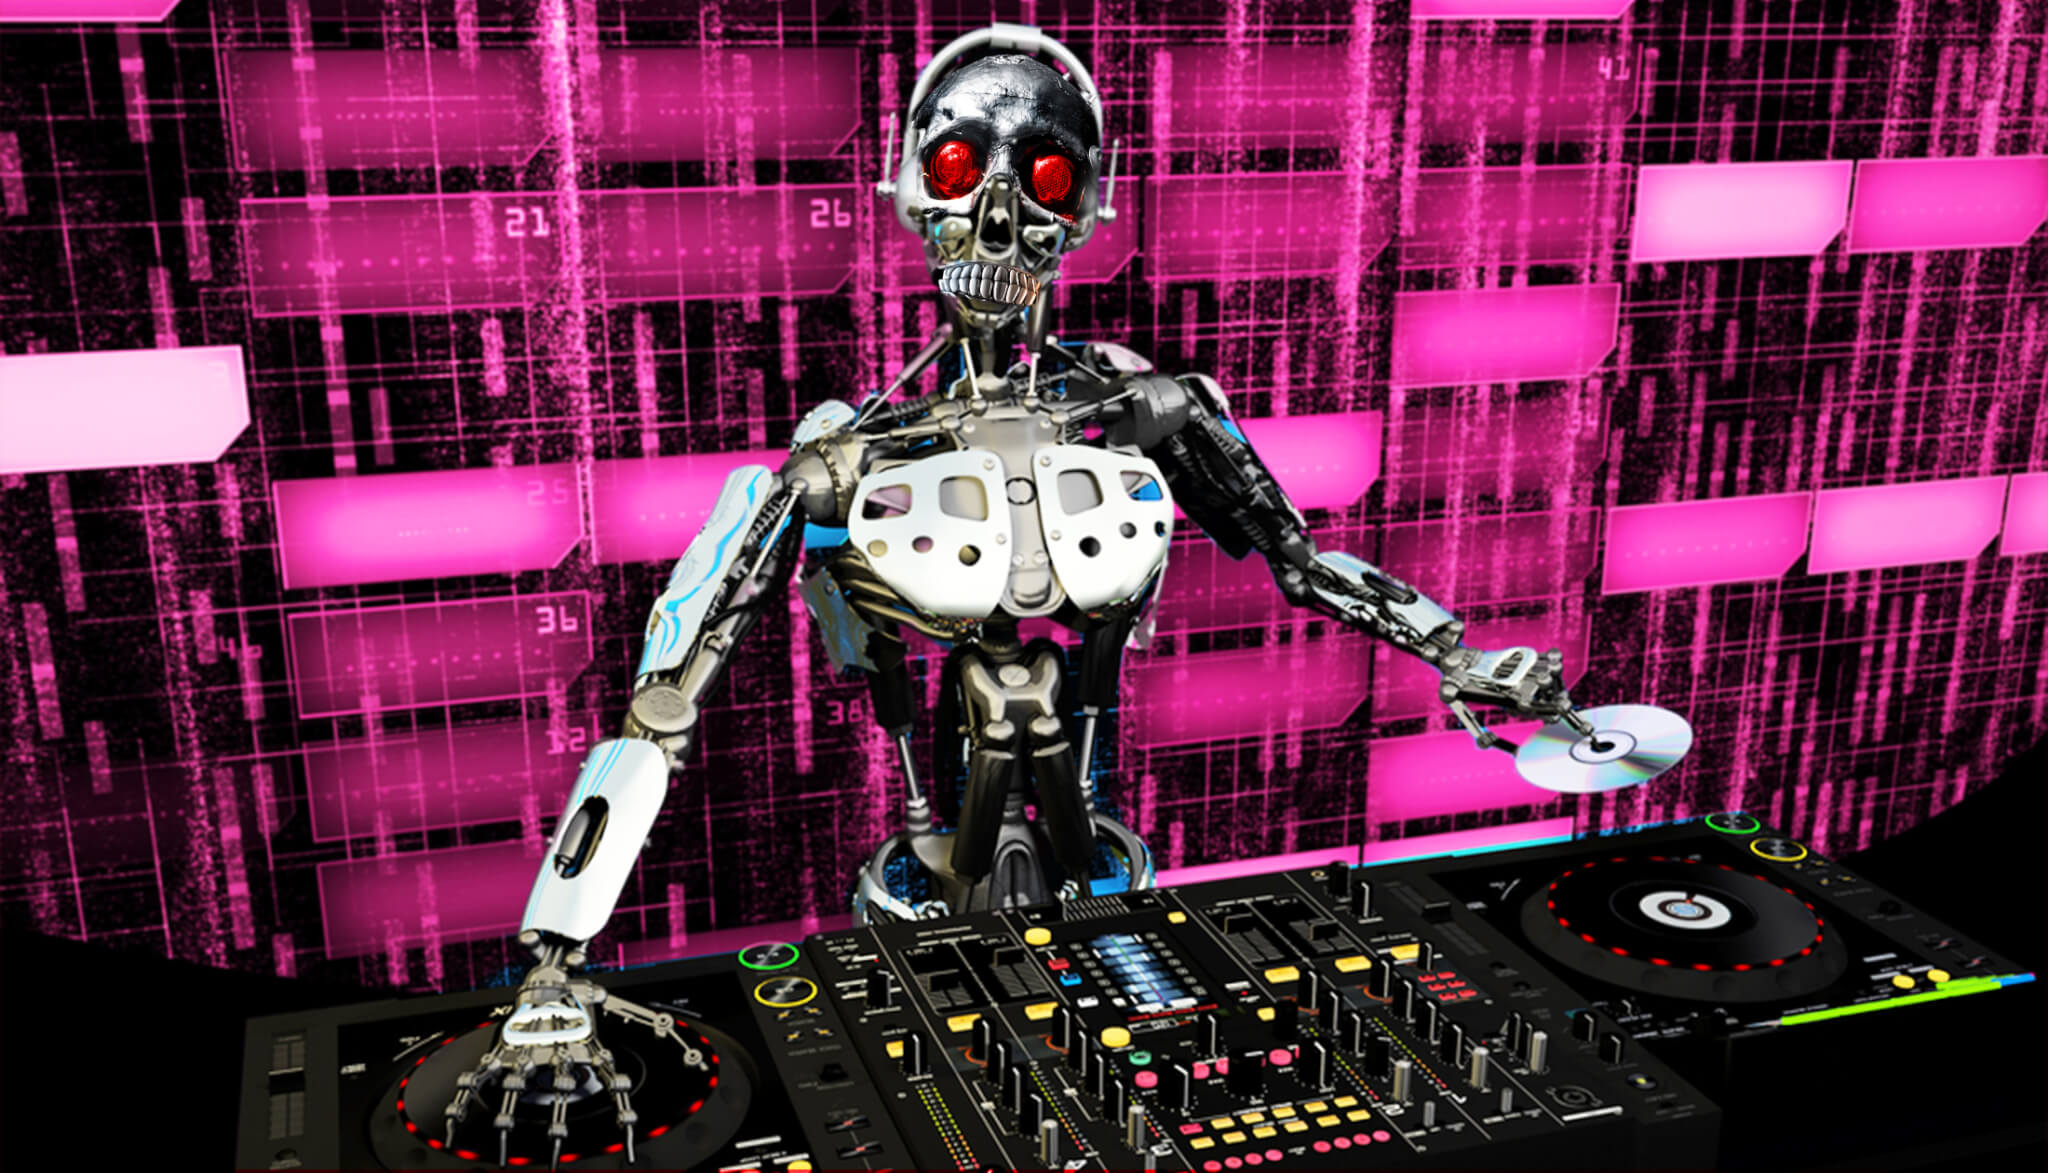
\includegraphics[width=\textwidth]{robot.jpg}
    \caption*{image source: \url{https://www.electronicbeats.net/app/uploads/2018/03/robotdj_spotify.jpg}}
\end{figure}

\vspace{-1em}

\begin{columns}[T]

%%%%%%%%%%%%%%%%%%%%%%%%%%%%%%%%%%%%%%%%%%%%%%%%%%%%%%%%%%%%%%%%%%%%%%%%%%%%%%%%
%%%%%%%%%%%%%%%%%%%%%%%%%        MIDDLE  COLUMN        %%%%%%%%%%%%%%%%%%%%%%%%%
%%%%%%%%%%%%%%%%%%%%%%%%%%%%%%%%%%%%%%%%%%%%%%%%%%%%%%%%%%%%%%%%%%%%%%%%%%%%%%%%

\begin{column}{0.486\textwidth}

%---RNN-based Approaches------------------------------------------------------------------

\begin{block}{RNN-based Approach}
\begin{minipage}[]{\blocktextwidth}
Recurrent Neural Networks (RNNs) are used to process sequences of data.
Output data is not only based upon input data, but also on a hidden state vector, that encodes previous input.

A promising candidate for music generation is the \textbf{SampleRNN}~\cite{mehri2016samplernn} (see Figure below).
Stacked \emph{Frame-Level Modules} with different fields of perception are used to capture temporal context over different time periods (tier 2 and 3).
A \emph{Sample-Level Module} puts their state vector into consideration as well as the current input sample to generate a probability distribution for the next sample (tier 1).
Originally tested only for piano music, \cite{zukowski2018generating} and \cite{carr2018generating} showed, that SampleRNN is especially good to generate loud music genres, like Metal and Dark Ambient.
Its biggest drawback is, that sample quality varies strongly even after days of training.
\begin{figure}[ht]
    \label{fig:samplernn}
    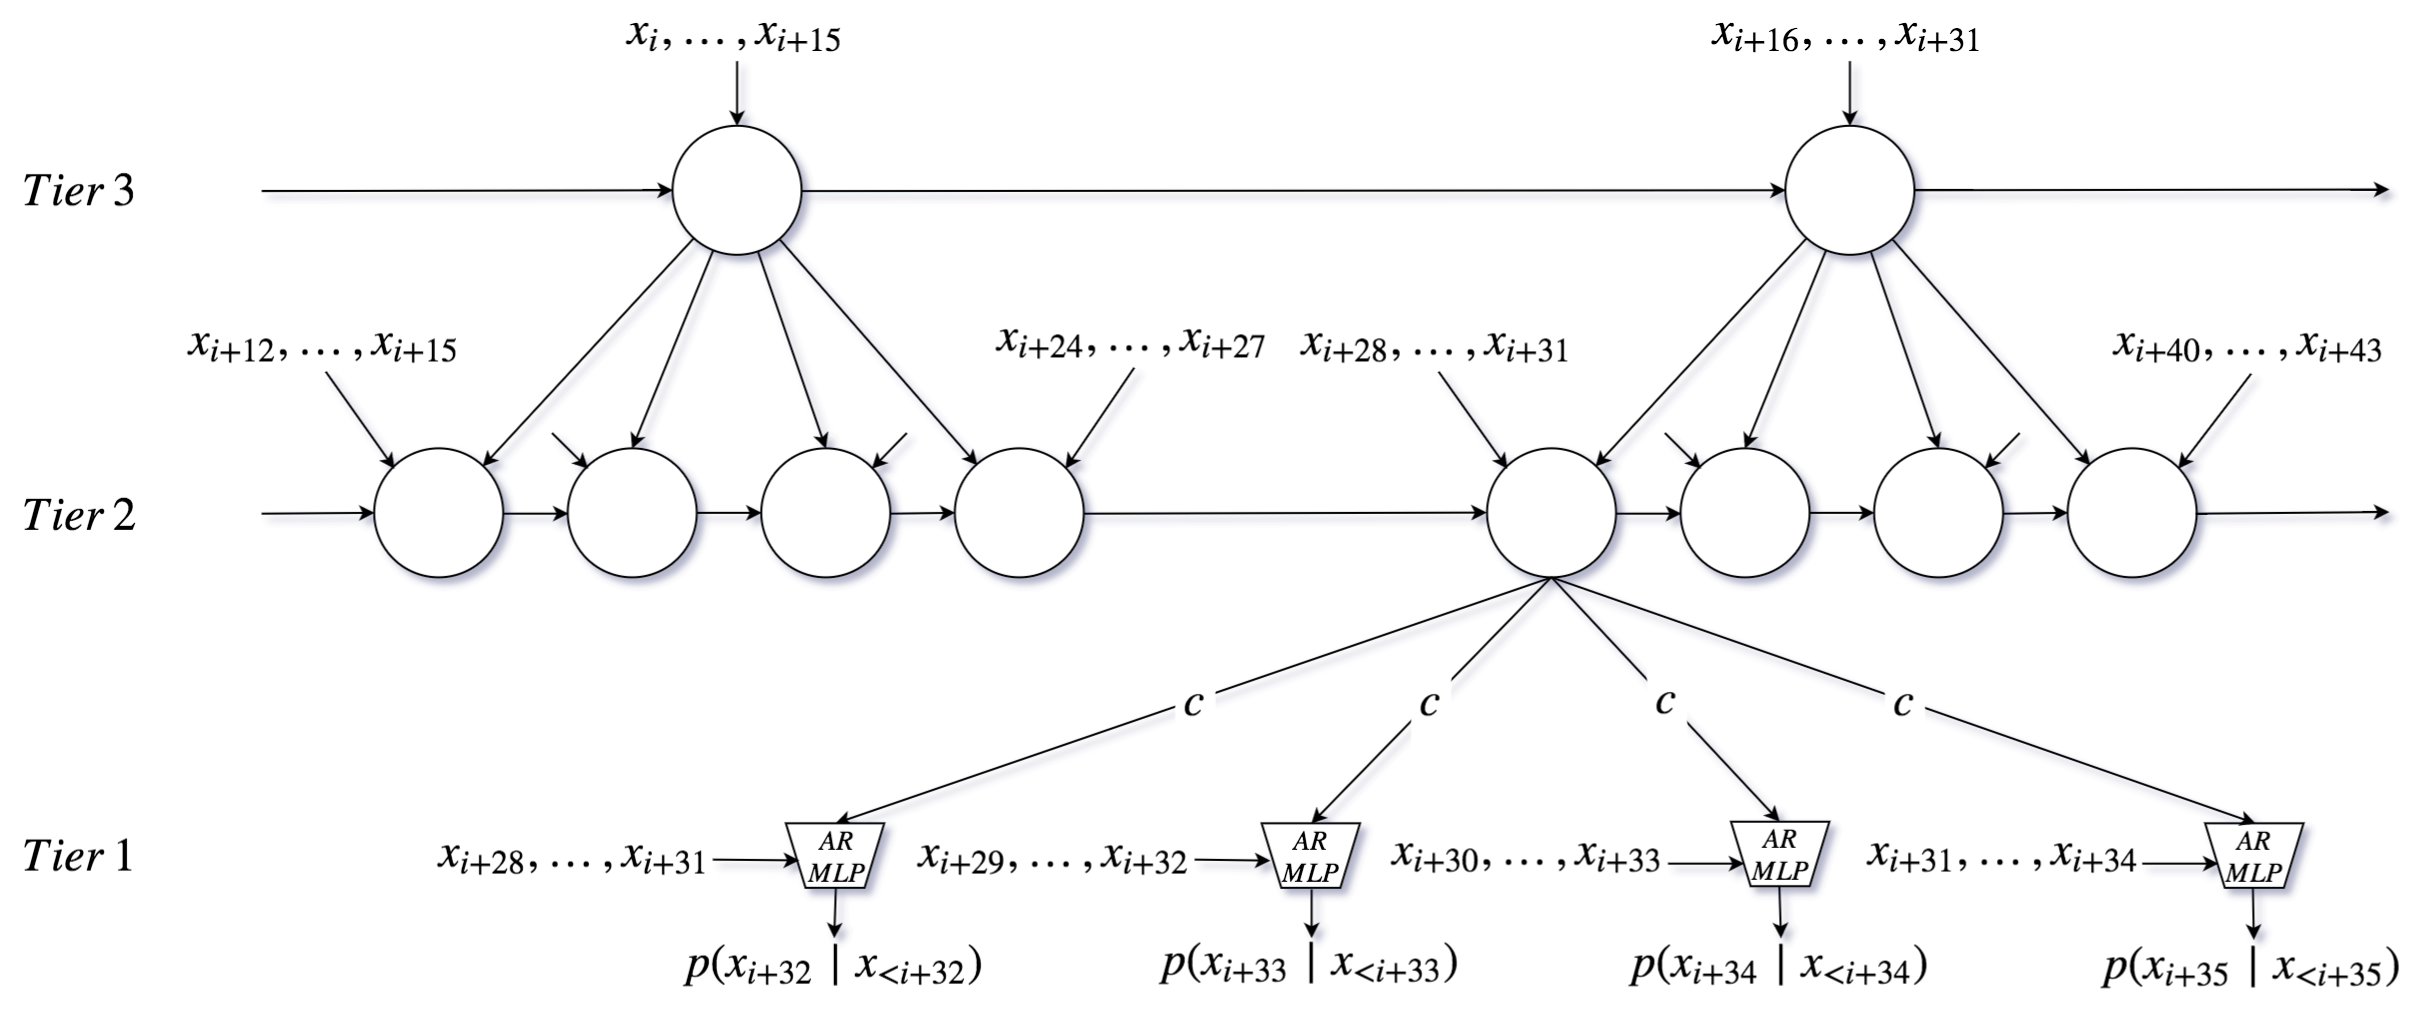
\includegraphics[height=92mm]{samplernn.png}
    \caption*{simplified architecture of the SampleRNN network}
\end{figure}
\end{minipage}
\end{block}




%\vspace{0.8em}

%\begin{figure}
%\centering\tiny
%\adjustbox{width=0.9\columnwidth,trim=0em 1em 3em 2em}{\input{cvmr}}
%\end{figure}

%\vspace{1em}


%---GAN-based----------------------------------------------------------------

\begin{block}{GAN-based Approach}
\begin{minipage}[]{\blocktextwidth}
Generative Adversarial Neural Networks (GANs) are a new kind of architecture.
While a Generator network tries to produce realistic data, a Discriminator network aims to separate real from generated data.

Donahue et al. proposes \textbf{SpecGAN}, which is based on convolutions of spectrogram images and \textbf{WaveGAN}, which is based on 1D convolutions on raw audio data~\cite{donahue2018adversarial}.
Engel et al. suggests to use progressively growing GANs to improve training stability~\cite{engel2019gansynth}.
This \textbf{Gansynth} network also works on spectrogram images.
However, all of these approaches only work on fixed length audio input and output, which can be a drawback due to limited memory.

\end{minipage}
\end{block}




%-------------------------------------------------------------------------------

\end{column}

\hfill

%%%%%%%%%%%%%%%%%%%%%%%%%%%%%%%%%%%%%%%%%%%%%%%%%%%%%%%%%%%%%%%%%%%%%%%%%%%%%%%%
%%%%%%%%%%%%%%%%%%%%%%%%%%%%%%%%%%%%%%%%%%%%%%%%%%%%%%      RIGHT  COLUMN      %
%%%%%%%%%%%%%%%%%%%%%%%%%%%%%%%%%%%%%%%%%%%%%%%%%%%%%%%%%%%%%%%%%%%%%%%%%%%%%%%%

\begin{column}{0.486\textwidth}


%---Progress-----------------------------------------------------------------


\begin{block}{Progress}
\begin{minipage}[]{\blocktextwidth}
\begin{itemize}[leftmargin=*,labelindent=0pt,label={\color{black!40}$\bullet$}]
\item{Implementation and training of WaveGAN}
\item{Update and Training of an outdated \mbox{SampleRNN} implementation}
\end{itemize}
\end{minipage}
\end{block}

\vspace{-1em}

%---FUTURE-WORK-----------------------------------------------------------------


\begin{block}{Future Work}
\begin{minipage}[]{\blocktextwidth}
\begin{itemize}[leftmargin=*,labelindent=0pt,label={\color{black!40}$\bullet$}]
\item{Implement and train more architectures}
\item{Directly compare generated music from different networks that were trained on the same dataset}
\end{itemize}
\end{minipage}
\end{block}






%---REFERENCES------------------------------------------------------------------

\vspace{-1em}
{
\setbeamercolor{block title}{fg=myfg,bg=white} % Change the block title color
\setbeamercolor{block body}{fg=myfg,bg=white} % Change the block title color

\begin{block}{References}
\vspace{-.5\baselineskip}
\bibliographystyle{unsrt}
\scriptsize{\bibliography{./literatur}}
\end{block}
}


%-------------------------------------------------------------------------------

\end{column}
\end{columns}

%-------------------------------------------------------------------------------

\end{column} % End of the second column
\end{columns} % End of all the columns in the poster


%-------------------------------------------------------------------------------

\end{frame} % End of the enclosing frame

\end{document}
